
\chapter{Background and literature review}

\section{The Otter USV and its sensor package}

Being able to sense the surrounding environment is crucial for any autonomous robot. In maneuvering, taking the appropriate action is highly dependent on having up-to-date and accurate information about the surroundings. The USV's sensors is what translates the environmental conditions into signals suitable for processing. Selecting the proper sensors is therefore critical, as it directly affects the quality of environmental information available, and consequently the maneuvering performance. This section will present the Otter USV and the sensors that are used in order to sense the surrounding environment and localize the USV.

\subsection{The Otter USV}

The experimental platform used in this thesis is the Otter USV \citep{website:MR}, an easily deployable system for bathymetric surveys developed by Maritime Robotics. The USV has a small footprint of $200$ x $105$ x $\SI{85}{\cm}$ and a weight of about $\SI{95}{\kilogram}$. It has a typical operating speed of about $\SI{2}{knots}$, and is propelled by a set of dual electrical fixed thrusters. The USV's stable catamaran design offers a payload capacity capable of supporting a multitude of different sensor configurations. The Otter USV is depicted in \figref{fig:experimental_platform}. 

\begin{figure}[h!]
    \centering
	\makebox[\linewidth][c]{
	\begin{subfigure}[b]{0.5\textwidth}
		\includegraphics[width=1\linewidth]{fig/lit_rev/infographics.jpg}
		\caption{}
		\label{fig:infographics}
	\end{subfigure}
	\begin{subfigure}[b]{0.5\textwidth}
		\includegraphics[width=1\linewidth]{fig/lit_rev/otter1}
		\caption{}
		\label{fig:otter_with_lidar}
	\end{subfigure}
	}
	\caption[Specifications of the Otter USV.]{(a) Specifications of the Otter USV, courtesy of Maritime Robotics. (b) The Otter USV equipped with a lidar in Trondheim harbor.} \label{fig:experimental_platform}
\end{figure}

\subsection{Relevant sensors}

\subsubsection{Lidar}

Lidar (also called LIDAR or LiDAR) stands for light detection and ranging, and is a method that uses light to measure the distance to a target \citep{wiki:lidar}. This is done by emitting laser pulses and measuring the time it takes for the pulse to be reflected. Measuring the distance in a wide range of directions allow lidars to make accurate and precise depictions of the surroundings, as illustrated in \figref{fig:lidar}.

\begin{figure}[h!]
    \centering
	\makebox[\linewidth][c]{
	\begin{subfigure}[b]{0.5\textwidth}
		\includegraphics[width=1\linewidth]{fig/lit_rev/lidar_sim.jpg}
		\caption{}
		\label{fig:lidar_rays}
	\end{subfigure}
	\begin{subfigure}[b]{0.5\textwidth}
		\includegraphics[width=1\linewidth]{fig/lit_rev/lidar_scan}
		\caption{}
		\label{fig:lidar_scan}
	\end{subfigure}
	}
	\caption[Illustration of a laser scan.]{(a) The USV in a simulated environment with obstacles. (b) The laser scan created by the lidar depicts an accurate mapping of the surroundings.}
	\label{fig:lidar}
\end{figure}

The range, resolution, and field of view vary a lot between different types of lidars. However, even low-cost 2D lidars can be used for navigation, for example in vacuum cleaners such as the Roborock S6 \citep{website:roborock}. A low-cost 2D lidar was also used successfully by \citet{Ueland2016} on a marine vessel to explore and navigate in a basin with unknown obstacles. A significant drawback of 2D lidars is that obstacles that occur either above or below the sensor's horizontal scan plane will not be detected. To account for this issue, \citet{Spange2016} incorporated the use of acoustic proximity sensors, which solves the issue inside the range of the proximity sensors. Both of the works by \citet{Spange2016} and \citet{Ueland2016} were performed in a basin where the lidar was largely unaffected by roll and pitch motions caused by waves.

Examples of better and more expensive 2D lidars are those in use on the multipurpose unmanned ground vehicles (UGVs) by Clearpath robotics \citep{website:Clearpath}. Compared to the cheaper lidars, these usually offer a significant increase in range, resolution and outdoor availability. State-of-the-art 3D lidars offer even more detailed depictions of the surrounding environment and avoid the issue of a single scan plane as in 2D lidars, but at the cost of a significant price increase. High-end lidars like this can be used in applications where the requirements to accuracy and precision are incredibly high, such as terrain mapping and self-driving cars. See for instance the Velodyne Puck \citep{website:VLP} and the YellowScan Surveyor \citep{website:YellowScan} lidars.

%% which to buy?
%The Otter USV does not require a very detailed mapping of the environment, it just needs enough detail to be able to detect large obstacles (like boats and jetties) and avoid them. Keeping the costs of the USV to a minimum is also of interest. Consequently, only low-cost 2D lidars are relevant when considering the sensor suite for the USV. Many 2D lidars are intended mainly for indoor use, and therefore have rather limited ranges and poor performance in sunlight. The 2D lidars from Hokuyo are examples of this, e.g. the Hokuyo URG-04LX-UG01 \citep{website:Hokuyo}. A low-cost 2D lidar which combines both a reasonable range and outdoors availability, is the RPLIDAR from SLAMTEC \citep{website:Slamtec}. This lidar is the Otter USV's main source of information about the surrounding environment.

\subsubsection{IMU}

An inertial measurement unit (IMU) is a device that measures the angular rate, force and sometimes magnetic field \citep{wiki:imu}. There are three main types of motion sensor devices in an IMU, and that is an accelerometer, gyroscope, and magnetometer. IMUs often contain some software that combines these measurements in order to provide orientation and heading, resulting in an attitude and heading reference system (AHRS). If the IMU has software that also calculates the position relative to a global reference frame, it is often called an inertial navigation system (INS) \citep{wiki:ins}. As with lidars, IMUs come with varying quality. Examples of cheap IMUs are the ones from SparkFun Electronics \citep{website:sparkfun}, while the very accurate POS MV \citep{website:applanix} system from Applanix is a much more accurate and expensive solution.

\subsubsection{GNSS}

Global navigation satellite system (GNSS) is a navigation system that uses satellites to provide geo-spatial positioning \citep{wiki:gnss}. GNSS allows small electronic receivers to determine their latitude, longitude, and altitude/elevation with high precision (within a few meters) using positioning and timing data transmitted from satellites. Popular publicly available GNSS systems include GPS, GLONASS, and Galileo. GNSS receivers are found many places such as in phones and watches, and are readily available at many online electronics stores \citep{website:sparkfun}. With more advanced RTK GNSS solutions, the precision of GNSS positioning can be increased to centimeter level accuracy \citep{wiki:rtk}, which is often important in applications such as land surveys and hydrographic surveys.

\subsubsection{MBES}

A multibeam echosounder (MBES) is a type of downward-looking sonar that is frequently used to map the seabed \citep{wiki:mbes}. The MBES is usually mounted on a ship's hull, and emits sound waves in a fan shape beneath the ship. The time it takes for the sound waves to bounce off the seabed and return to a receiver on the MBES, is used to determine water depth. This gives an accurate depiction of the seabed directly beneath the ship, see \figref{fig:mbes}.

\begin{figure}[h!]
    \centering
	\includegraphics[width=0.5\linewidth]{fig/lit_rev/mbes}
	\caption[Multibeam echosounder measurement of the seabead.]{A multibeam echosounder measures the depths in a swath beneath the ship. Visualized by Maritime Robotics' Vehicle Control Station.}
	\label{fig:mbes}
\end{figure}

There are several use cases for multibeam echosounders, and the field of view, depth range and resolution vary accordingly. The NORBIT iWBMS is an example of a compact and high resolution sonar for shallow water mapping, and can operate in depth ranges of $0.2$ -- $275$ meters \citep{website:norbit}. Other sonars, like the Kongsberg Maritime EM 124 are meant to operate at full ocean depths, and can handle depth ranges of $20$ - $11000$ meters \citep{website:km}.

\section{Partitioning of the operational workspace}

The operational workspace of a robot is the space in which the robot is operating. In the case of the Otter USV, the workspace is the reachable portion of the desired survey area. Partitioning the workspace then becomes the task of splitting the workspace into smaller, more manageable regions that are better suited for path planning. The choice of a partitioning strategy is an important part of CCPP, and is therefore given a thorough review here.

%The survey \citep{Galceran2013} summarizes many partitioning methods for CCPP.

\subsection{Grid-based decomposition}

In grid-based decomposition, the workspace is decomposed into a collection of uniform cells ordered in a grid. In this representation, each cell represents a small region of space in the real world, and is usually the size of the robot's footprint, end-effector, or observation sensor's coverage range. This makes it very suitable for CCPP, because when all cells in the grid are covered, complete coverage is achieved. Grid-based decomposition is, however, an approximate representation of the workspace. If the area a cell represents is only partially covered by an obstacle in the real world, the entire cell is often considered as an obstacle. Some grid-based decomposition methods are illustrated in \figref{fig:grid_shapes}.

\begin{figure}[h!]
    \centering
	\makebox[\linewidth][c]{
	\begin{subfigure}[t]{0.5\textwidth}
		\includegraphics[width=1\linewidth]{fig/lit_rev/square_cell1}
		\caption{Square cell decomposition \citep{Galceran2013}. Obstacles are outlined by the dashed lines, and the colored cells are considered obstacles.}
		\label{fig:grid_square}
	\end{subfigure}
	\quad
	\begin{subfigure}[t]{0.5\textwidth}
		\includegraphics[width=1\linewidth]{fig/lit_rev/circular_cell}
		\caption{Circular disk decomposition \citep{guo2004coverage}.}
		\label{fig:grid_circular}
	\end{subfigure}
	}
	\makebox[\linewidth][c]{
	\begin{subfigure}[t]{0.5\textwidth}
		\includegraphics[width=1\linewidth]{fig/lit_rev/triangular_cell}
		\caption{Triangular cell decomposition \citep{oh2004complete}. Colored rectangle represents obstacles.}
		\label{fig:grid_triangular}
	\end{subfigure}
	}
	
	\caption{Grid-based decomposition methods.}
	\label{fig:grid_shapes}
\end{figure}

Many CCPP methods use a grid-based decomposition in their partitioning of the workspace. The grid cells are often square, as in the methods by \citet{Viet2013} and \citet{yang2004neural}. However, other shapes are also used, such as circular disks \citep{guo2004coverage} and triangles \citep{oh2004complete}. Decomposition into circular disks with the coverage range as the radius of the circles, is motivated by the fact the it will sometimes give a more correct representation of the covered area compared to squares. Circular disk decomposition has been used in several CCPP methods, such as \citet{guo2006complete} and \citet{Scibilia2012}. The triangular cells used by \citet{oh2004complete} offers an advantage over other shapes in that each cell has 12 neighboring cells, resulting in more directions for movement between neighboring cells.

An advantage of grid-based decomposition, is that a grid-map is easy to create and maintain in an implemented system. It is easily represented in a simple array-structure, which most programming languages have access to. One of the downsides of grid-based decomposition is that it is approximate, and most CCPP methods using grids are therefore resolution-complete \citep{Galceran2013}. That is, the completeness of the methods depend on the resolution of the grid map, as seen in \figref{fig:grid_square}. Another disadvantage is that the requirement to memory becomes large in big workspaces with very small cell sizes. Grid-based decomposition also requires accurate localization and mapping in order to be able to distinguish between adjacent grid cells.

%This is because grid-based approaches require a resolution accurate enough to capture the most important details of the world \citep{thrun1998learning}.

\subsection{Morse-based cellular decomposition}

%See here: \citep{Galceran2013}.

\citet{acar2002morse} introduced the term Morse decompositions as a class of exact cellular decomposition whose cells have a simple structure that can be readily covered. In Morse-based cellular decomposition, the workspace is partitioned into non-overlapping cells that, together, exactly cover the workspace. Thus, exact cellular decomposition. The cells themselves are created based on critical points of Morse functions. By choosing different functions, different cell shapes are obtained. These cells are not uniform in size or shape as in grid-based partitioning, but rather shaped such that each cell itself can be covered by a simple motion. An example of a simple motion is the boustrophedon motion, i.e. a simple back-and-forth lawnmower pattern. Complete coverage is then achieved by covering each individual cell with a simple motion.



The chosen Morse function defines what Acar terms a slice function, and this slice is swept through the target space. When the sweep line encounters an obstacle with a surface normal perpendicular to the sweep line, a critical point is found. A vertical sweep line results in a boustrophedon decomposition \citep{choset2000exact}. \figref{fig:morse_crit} shows the online detection of a critical point and thus the edge of a cell. \figref{fig:morse_cells} shows a complete exact cell decomposition of a workspace.

\begin{figure}[h!]
    \centering
	\makebox[1.0\linewidth][c]{
	\begin{subfigure}[t]{0.5\textwidth}
		\includegraphics[width=1\linewidth]{fig/lit_rev/morse_crit}
		\caption{A critical point detected by a robot moving along the sweep line \citep{Galceran2013}.}
		\label{fig:morse_crit}
	\end{subfigure}
	\quad
 	\begin{subfigure}[t]{0.5\textwidth}
		\includegraphics[width=1\linewidth]{fig/lit_rev/morse_cells}
		\caption{Cell decomposition of a workspace \citep{acar2006sensor}.}
		\label{fig:morse_cells}
	\end{subfigure}
 	}
	\caption{Morse-based cellular decomposition with a vertical sweep line.}
	\label{fig:morse_decomp}
\end{figure}

The CCPP method by \citet{acar2002sensor} is an example of a method that uses Morse-based cellular decomposition. This is an online method that, upon the detection of critical points while moving through the workspace, creates and modifies cells. \citet{acar2006sensor} takes this approach one step further by combining Morse-based cellular decomposition with generalized Voronoi diagrams. The Voronoi diagrams are used for representing narrow or cluttered spaces, while Morse-based cellular decomposition is used for open spaces. This allows for more efficient coverage for certain types of robots and applications.

\section{Relevant methods for CCPP} \label{sec:lit-rev-ccpp}

There are some works in the literature that address the problem of CCPP for seabed coverage. \citet{galceran2013planning} is an offline CCPP method for AUVs that takes a bathymetric map as input and generates complete coverage paths for in-detail inspections of the ocean floor. \citet{williams2010optimal} detects underwater mines with an AUV by covering an area by parallel tracks with varying track-spacing. Another method by \citet{paull2013sensor} considers online CCPP for mine countermeasures with AUVs. These methods all operate on AUVs, and their main focus is on effective mapping of the seabed. However, online obstacle avoidance is not considered in any of them.

\citet{galceran2012efficient} proposed an efficient offline method for ASVs and AUVs that minimizes the amount of coverage overlap. Given a prior depth map, the method starts by segmenting the target area into regions of similar depth. Each of these regions are then handled as a separate coverage problem and, assuming no obstacles in the region, covered with simple parallel back-and-forth laps. Since the spacing between each lap is constrained by the shallowest point on the surface, the similar-depth regions reduce the coverage overlap. They further reduce coverage overlapping by choosing a sweeping direction inside each of these regions that is oriented perpendicular to the seafloor surface gradient, thus minimizing the difference between the shallowest and deepest point in one lap. Lastly, the inter-lap spacing is maximized on a lap-by-lap basis where the spacing is determined by the shallowest point on the current lap. The complete coverage paths generated by this method is shown in \figref{fig:galceran_ccpp}.

\begin{figure}[h!]
    \centering
	\includegraphics[width=0.5\linewidth]{fig/lit_rev/galceran_ccpp}
	\caption[Complete coverage paths for regions segmented by similar depth.]{Complete coverage paths for regions segmented by similar depth \citep{galceran2012efficient}.}
	\label{fig:galceran_ccpp}
\end{figure}

Most CCPP methods are developed for use with fixed size sensors or end-effectors, such as those found in vacuum cleaners, lawnmowers or painting robots. The comprehensive survey by \citet{Galceran2013} reviews many of these, and most of them use some sort of boustrophedon motions. Other methods, like \citet{yang2004neural} and \citet{Scibilia2012}, use a topologically organized neural network to plan the paths. While these methods do not address the topic of seabed mapping with a variable coverage range sensor, they do address the problem of obstacle avoidance in unknown environments. One method that makes use of boustrophedon motions, is the BA* method described in \citet{Viet2013}. In this method, the operational workspace is partitioned into uniform square grid cells. The method constructs boustrophedon motions by moving between cells in a north-south-east-west priority. When the robot gets stuck, it uses an A* search to backtrack to another starting point where a new boustrophedon motion is started. The paths generated by the method is shown in \figref{fig:ba_star}. 

\begin{figure}[h!]
    \centering
	\includegraphics[width=0.5\linewidth]{fig/lit_rev/ba_star}
	\caption[Complete coverage with boustrophedon motions and backtracking with A* search.]{Complete coverage with boustrophedon motions and backtracking with A* search \citep{Viet2013}.}
	\label{fig:ba_star}
\end{figure}

\section{Feasible path design}

Most CCPP methods generate paths as waypoints, or as straight-line segments between waypoints. This is perfectly fine for robotic applications where the cost of repeatedly starting, stopping and in-place turning is low, such as lawn mowing and floor cleaning. For other applications, especially those involving underactuated USVs, this is far less favorable due to an increase in factors such as power consumption and time duration. In these cases, it is desirable with a feasible path that takes into account the kinematic constraints of the robot.

Connecting points with feasible paths can be achieved in several ways, each with its own advantages and disadvantages. The different approaches can usually be distinguished into two main categories: combining straight lines and arc segments, or using splines \citep{lekkas2014guidance}. % In this thesis, straight lines and arc segments are used. 
The main disadvantage of using straight lines and arc segments is the curvature discontinuity which occurs between two consecutive path segments. On the other hand, the constant curvature of these paths allows for smaller variations in the control outputs compared to splines. Splines are smooth, but have an always varying curvature which means the control output is changing all the time.

%Moving on straight lines and arc segments also means fewer zig-zag turns between points, ensuring a more stable course. This is an advantage in applications like seabed mapping, where an accurate course estimate is important for the quality of measurements.

\subsection{Polynomial approximation}

\citet{guo2006complete} proposed an approach for polynomial approximation using a rolling window of six waypoints, see \figref{fig:poly_approx}. A smooth path is sequentially generated between the third and fourth waypoint. Consequently, this method requires planning at least three waypoints ahead in time. The approach generates three cubic polynomials from the first four points, middle four points, and last four points. These three polynomials are then used to obtain the first and second derivatives of the line-segment between the third and fourth waypoint. These, in turn, can be used as boundary conditions in order to obtain a fifth order polynomial which connects the third and fourth waypoint. Consequently, the resulting path is guaranteed to have continuous second-order derivatives.

\begin{figure}[h!]
    \centering
	\includegraphics[width=0.5\linewidth]{fig/lit_rev/poly_approx}
	\caption[Polynomial approximation of a 6-point rolling window.]{Polynomial approximation of a 6-point rolling window \citep{guo2006complete}.}
	\label{fig:poly_approx}
\end{figure}

\subsection{Dubins path}

Dubins path is the shortest path for a Dubins vehicle between two points with a constraint on average curvature, and with prescribed initial and terminal positions and tangents \citep{dubins1957curves}. Dubins vehicle is defined as a non-holonomic vehicle that is constrained to move along planar paths of bounded curvature, and can only travel forward along the path. The generated Dubins path is composed only of circular arcs and line segments as shown in \figref{fig:dubins_path}. By using a robot's minimum turning radius in the generation of the Dubins path, the feasibility of the path is guaranteed.

\begin{figure}[h!]
    \centering
	\makebox[1.0\linewidth][c]{
	\begin{subfigure}[t]{0.5\textwidth}
		\includegraphics[width=1\linewidth]{fig/lit_rev/dubins1}
		\caption{}
		\label{fig:dubins1}
	\end{subfigure}
	\quad
 	\begin{subfigure}[t]{0.5\textwidth}
		\includegraphics[width=1\linewidth]{fig/lit_rev/dubins2}
		\caption{}
		\label{fig:dubins2}
	\end{subfigure}
 	}
	\caption[Dubins path.]{Dubins path, courtesy of Wikipedia.}
	\label{fig:dubins_path}
\end{figure}

The guidance system proposed by \citet{Scibilia2012} generates feasible paths for AUVs by using what is referred to as simple Dubins paths. By removing the constraint on the terminal heading of a Dubins path, the path is simplified considerably. The path can further be simplified by requiring a minimum feasible turning radius that is smaller than half the distance between the start and end point. The shortest path can then be described by what is referred to as a simple Dubins path, i.e. a single turn followed by a straight-ahead movement. A simple Dubins path is shown in \figref{fig:simple_dubins_path}, the terminal heading is determined from the path.


\begin{figure}[h!]
	\centering
	\makebox[1.0\linewidth][c]{
	\begin{subfigure}[t]{0.5\textwidth}
		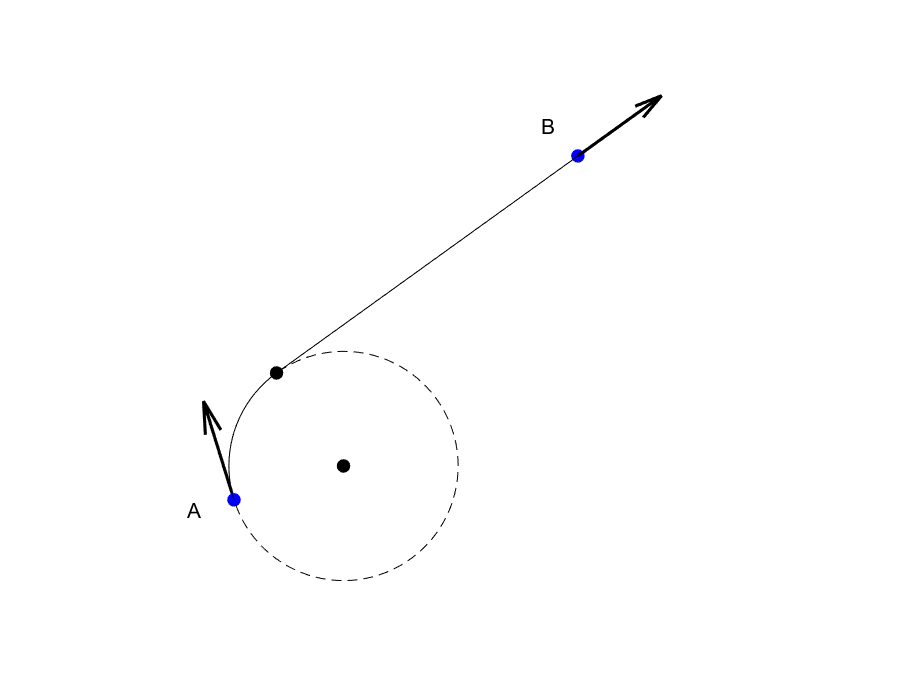
\includegraphics[width=1\linewidth]{fig/lit_rev/simple_dubins_path}
		\caption{}
		\label{fig:simple_dubins1}
	\end{subfigure}
	\quad
 	\begin{subfigure}[t]{0.5\textwidth}
		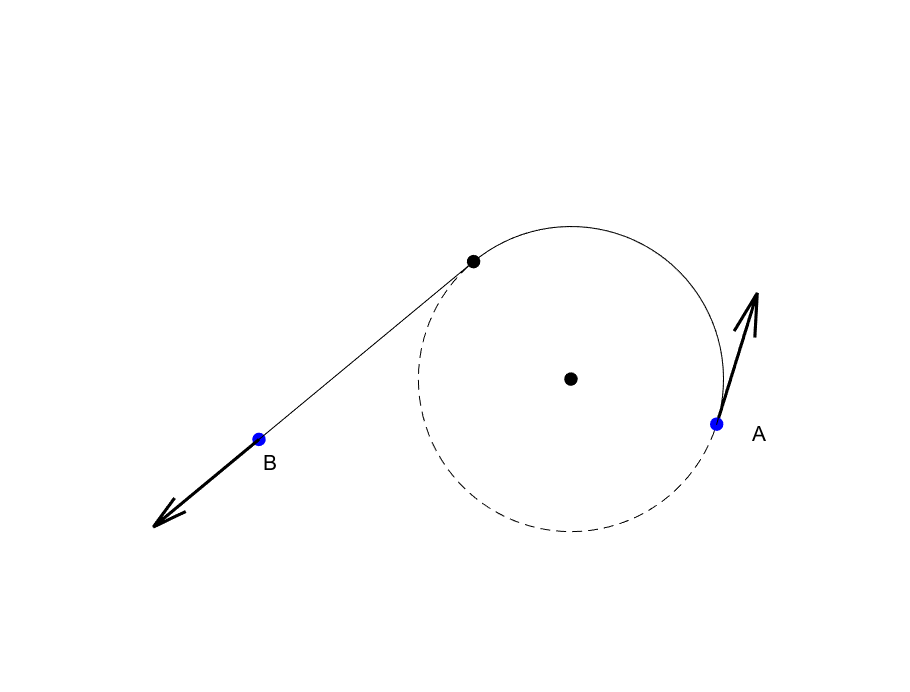
\includegraphics[width=1\linewidth]{fig/lit_rev/simple_dubins_path2}
		\caption{}
		\label{fig:simple_dubins2}
	\end{subfigure}
 	}
	\caption{Simple Dubins path.}
	\label{fig:simple_dubins_path}
\end{figure}


\subsection{Bezier curves}

Bezier curves are defined by a set of control points, but the curve itself does not pass through these points, as shown in \figref{fig:bezier_curve}. Bezier curves have several interesting and useful properties for path planning \citep{choi2008path}. For instance, together the control points define a polygon, and the Bezier curve will always be contained within the convex hull of this polygon. Another useful property is that the first and last points on the curve are coincident with the first and last control points. Furthermore, the tangents of the curve at these points are also coincident with the first and last line segments generated by subsequent control points. 

\begin{figure}[h!]
	\centering
	\includegraphics[width=0.5\linewidth]{fig/lit_rev/bezier_curve}
	\caption[Bezier curve.]{Bezier curve, courtesy of Wikipedia.}
	\label{fig:bezier_curve}
\end{figure}

\citet{jolly2009bezier} presented an approach to path planning for soccer robots based on Bezier curves. In robot soccer, it is important to hit the ball from the correct direction, making Bezier curves an appropriate choice. While the intended application of the approach is in robot soccer, the generation of the Bezier curves in itself is applicable for other scenarios as well. The approach is based on the selection of four control points, as shown in \figref{fig:bezier_soccer}. The first and last control points are taken as the estimated position of the robot and the target. The second control point is located based on the estimated heading of the robot and a distance ($d_1$ in the figure). Similarly, the third control point is located based on the desired final heading and a distance ($d_2$ in the figure). The distances to the second and third control points are determined through an iterative optimization algorithm which takes into account the acceleration limits of the robot.

\begin{figure}[h!]
	\centering
	\includegraphics[width=0.5\linewidth]{fig/lit_rev/bezier_soccer.jpg}
	\caption[A Bezier curve ensuring that the robot hits the ball from the right direction in robot soccer.]{A Bezier curve ensuring that the robot hits the ball from the right direction in robot soccer \citep{jolly2009bezier}.}
	\vspace*{5.5in}
	\label{fig:bezier_soccer}
\end{figure}


